\section{Introduction}

The world is full of moving things, and increasingly, things know where they are. 
Ubiquitous sensor technologies, like GPS, combined with networked storage enables us to continually detect and archive spatial movement.
These myriad data points can answer questions of great value, including geospatial distributions, trends and traffic flows, popular restaurants, migration patterns and much more.

\begin{wrapfigure}{l}{0.42\textwidth}
  \centering
  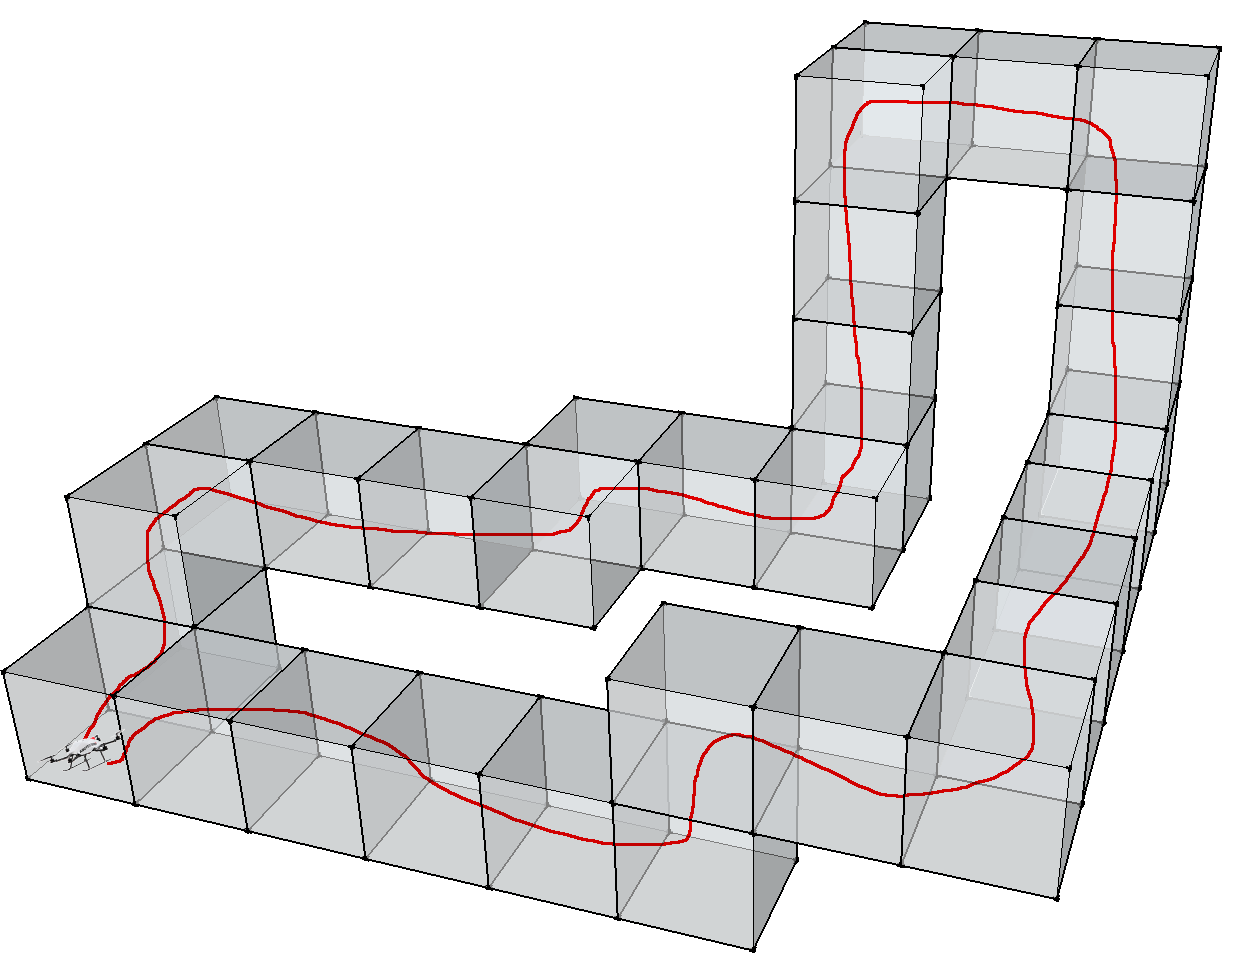
\includegraphics[width=0.42\textwidth]{./figures/path_overview}
  \caption{Unit cube space used in spatial abstraction.}
  \label{fig:unitCubes}
\end{wrapfigure}

However, we can be overwhelmed because we are ``drowning in data"~\cite{morse1993drowning}.
Further, it can be difficult to examine high-level relationships because points and lines are specific; the story is at the level of the forest and we can only see the trees.  
Often it is only feasible to analyze large data sets by choosing an appropriate level of abstraction.
The work presented here is about one such kind of abstraction.
We consider a ``spatial abstraction" where particular points in space-time are mapped to unit cubes, as shown in Fig.~\ref{fig:unitCubes}.
Using techniques inspired by software analysis, specifically Daikon invariants~\cite{kataoka2001automated}, we use trace data gathered as an object moves and explore the properties of movement of things at a higher level.

In this paper, we set forth our technique for abstracting away from particular points, 
implement our technique in a prototype tool, ``FuzzyCubicCrumbTeleportation", 
collect real movement data from a small flying robot, 
and validate our tools' ability to detect spatial properties on one or more actors.

The paper is organized as follows:
Section~\ref{sec:background} gives an overview of both spatial analysis and the Daikon invariants analysis tool;
Section~\ref{sec:method} describes the method of spatial abstraction, including defining terms and a table of formalized properties;
Section~\ref{sec:tool} provides an overview of our tool that implements this method of analysis;
Section~\ref{sec:experiments} shows an initial application of our tool to a real robotic system;
Section~\ref{sec:related} situates this work relative to other kinds of movement analysis;
Section~\ref{sec:conclusion} summarizes this work and describes future lines of inquiry. 




